%&mybeamer
%\documentclass[ignoreonframetext,12pt]{beamer}
%\documentclass{mybeamer}

% Meta data
\author{Daniel Hoske}
\title{Book Embedding with Fixed Page Assignments}
\date{23rd October 2012}
\institute{Department of Informatics, Institute of Theoretical Computer Science\\
Advisors: Dipl.-Inform. Thomas Bläsius, Dr. Ignaz Rutter}


\newcommand{\SEFE}{\prob{sefe}}
\newcommand{\SEFECON}{\prob{connected-sefe}}
\newcommand{\PQ}{PQ\xspace}
\newcommand{\Q}{Q\xspace}
\newcommand{\PT}{P\xspace}

% Algorithmic problems
\newcommand{\prob}[1]{\textsc{#1}\xspace}
\newcommand{\probTwoSat}{\prob{2-sat}}
\newcommand{\probThreeSat}{\prob{3-sat}}
\newcommand{\probQTree}{\prob{q-tree-book-embedding}}
\newcommand{\probPTree}{\prob{p-tree-book-embedding}}
\newcommand{\probQTreeSat}{\prob{q-tree-2-sat}}
\newcommand{\probBookNormal}{\prob{not-fixed-book-embedding}}
\newcommand{\probBook}{\prob{book-embedding}}
\newcommand{\probBookConnected}{\prob{connected-book-embedding}}
\newcommand{\probBetween}{\prob{betweenness}}
\newcommand{\probBookOrder}{\prob{order-book-embedding}}
\newcommand{\probMatching}{\prob{perfect-matchings-book-embedding}}
\newcommand{\probNotMatching}{\prob{matchings-book-embedding}}
\newcommand{\probPQ}{\prob{simultaneous-pq-ordering}}
\newcommand{\probMul}{\prob{multiple-spine-embedding}}
\newcommand{\probThreeMatching}{\prob{3-perfect-matchings-book-embedding}}
\newcommand{\range}[1]{\{1, \dotsc, #1\}}
\newcommand{\newProb}[3]{%

\vspace{.5em}
\begin{block}{Problem: #1}
\emph{Given:} #2\\%
%\emph{Answer the question:} #3%
\emph{Question:} #3%
\end{block}
\vspace{.5em}
}    

% Tikz options
\tikzstyle{dashdot} = [dash pattern=on .8pt off 3pt on 4pt off 3pt]
\tikzstyle{edge1}=[red,dashed]
\tikzstyle{edge2}=[blue,dotted]
\tikzstyle{edge3}=[green,dashdot]
\tikzstyle{every node}+=[inner sep=0.5mm,minimum size=2.00mm,node distance=3em,thick]
\tikzstyle{every edge}+=[thick]
\tikzstyle{every arc}+=[thick]
\tikzstyle{every path}+=[thick]
\usetikzlibrary{svg.path,calc,decorations.pathreplacing,positioning,backgrounds}
\newdimen\XCoord
\newdimen\YCoord
\newcommand*{\ExtractCoordinate}[1]{\path #1; \pgfgetlastxy{\XCoord}{\YCoord};}%

\newcommand{\drawedges}[2][\empty]{
	\foreach \a/\b in {#2}{
		\draw[#1] (\a) edge (\b);
	}
}

% Semicircle through a and b
\newcommand{\semicircle}[2]{%
  \ExtractCoordinate{($ 0.5*($ (#2.north) - (#1.north) $) $)}
  \draw[thick] ($ (#2.north) $) arc (0:180:\XCoord);
}

\def\caption[#1]#2{}

\newcommand{\mytt}[1]{{\footnotesize \texttt{#1}}}

\newcommand{\solutionTri}[2]{
  \begin{figure}\centering
  \resizebox{#2}{!}{
  \begin{tikzpicture}
    \coordinate (1) at (0,0);
    \coordinate (2) at (60:8);
    \coordinate (3) at (8,0);
    
	\draw (1) -- (2)
	      (2) -- (3)
	      (3) -- (1);    
    
    \node (centre) at ($ 1/3*($ (1) + (2) + (3) $) $) {3 pages?};    
    
    \ifthenelse{#1 > 0}{\node (a) at ($ (2) + (0, .5) $) {$2$ pages: $\OO(n)$};}{}
    \ifthenelse{#1 > 1}{\node (b) at ($ (1) + (0, -.5)$) {$k$ connected pages: $\OO(kn)$};}{
                        \node[white] (b) at ($ (1) + (0, -.5)$) {$k$ connected pages: $\OO(kn)$};}
    \ifthenelse{#1 > 2}{\node (c) at ($ (3) + (0, -.5) $) {$k$ matchings: in NPC};}{}
    \ifthenelse{#1 > 3}{\node (d) at ($ 0.5*($ (3) + (centre) $) + (-.5,0) $) {$3$ perfect matchings?};}{}
    \ifthenelse{#1 > 4}{
      \node (e) at ($ (1) + (0,-1) $) {P-trees?};
      \node (f) at ($ (e) + (3,0) $) {Q-trees: $\OO(kn^2)$};
      \draw (e) -- (f);
    }{}
    
    \draw[draw=none, use as bounding box](-2,-2) rectangle (10,8);
  \end{tikzpicture}
  }
  \end{figure}
}

\newcommand{\resultFrame}[1]{
  \miniframesoff
  \begin{frame}{Results}
    \solutionTri{#1}{0.8\textwidth}
  \end{frame}
  \miniframeson
}

\begin{document}

\miniframesoff
\setbeamerfont{title}{size=\large}
\setbeamerfont{author}{size=\normalsize}
%\setbeamerfont{institute}{size=\normalsize}
\begin{frame}\titlepage\end{frame}

\begin{frame}{Page embedding}
\begin{definition}
\emph{Page embedding} is planar embedding with\\
      \begin{itemize}
        \item vertices on a line and
        \item edges in half-plane above the line
      \end{itemize}
\end{definition}

\begin{overprint}
\onslide<1>
\begin{figure}
\centering

\scalebox{0.5}{\begin{tikzpicture}

\draw[->,thin] (-1em,0) -- ++(9em, 0) node [right] {x};
\draw[->,thin] (-1em,0) -- ++(0,9em)  node [above] {y};

\node[fill=white] (1) {a};
\node[fill=white,right of=1] (2) {b};
\node[fill=white,right of=2] (3) {c};

\draw (1) edge [bend left] (2);
\draw (2) edge [bend left] (3);
\draw (1) edge [bend left] (3);
\end{tikzpicture}}

\end{figure}
Page embeddable = outerplanar
\onslide<2>
Page embeddable = outerplanar
\begin{figure}\centering
\resizebox{0.7\textwidth}{!}{
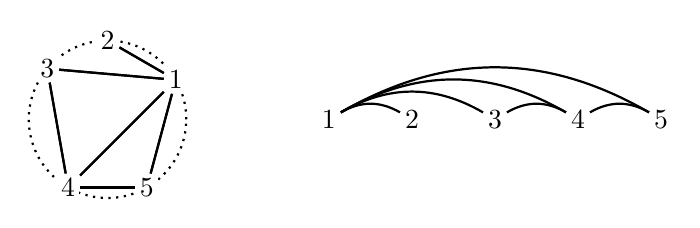
\begin{tikzpicture}
    \tikzstyle{every node}+=[fill=white]
	\draw[dotted] (0, 0) circle (1);
	\node (1) at (30:1) {1};
    \node (2) at (90:1) {2};
	\node (3) at (140:1) {3};
	\node (4) at (240:1) {4};
	\node (5) at (300:1) {5};
	\drawedges{1/2,3/4,1/3,1/4,1/5,4/5};
	\draw (1) -- (2);
	\draw (3) -- (4);
	\draw (1) -- (3);
	\draw (1) -- (4);
	\draw (1) -- (5);
	\draw (4) -- (5);
	
    \node[draw=none,fill=none] at (2.0,0) {{\Huge $\rightsquigarrow$}};	
	
	\begin{scope}[xshift=8em]
	\node (1) at (0, 0) {1};
	\node (2) [right of=1]{2};
    \node (3) [right of=2]{3};
	\node (4) [right of=3]{4};
	\node (5) [right of=4]{5};
    \drawedges[bend left]{1/2,3/4,1/3,1/4,1/5,4/5};		
	\end{scope}
\end{tikzpicture}
}
\end{figure}
\end{overprint}
\end{frame}

\begin{frame}{Book embedding}

\begin{definition}
\emph{Book embedding} of $G_i = (V, E_i)$, $i \in \range{k}$ consists of 
page embeddings for~$G_i$ with the same vertex positions.
\end{definition}

\begin{overprint}
\onslide<1>
\begin{figure}
\centering

\resizebox{0.6\textwidth}{!}{
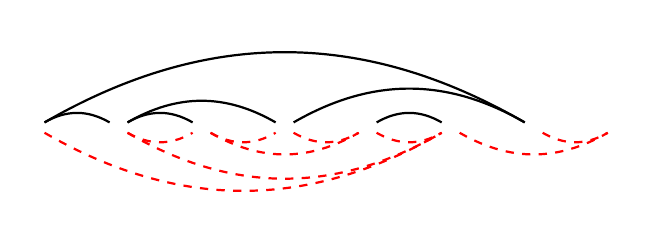
\begin{tikzpicture}
\node (1) {};
\node [right of=1] (2) {};
\node [right of=2] (3) {};
\node [right of=3] (4) {};
\node [right of=4] (5) {};
\node [right of=5] (6) {};
\node [right of=6] (7) {};
\node [right of=7] (8) {};

\drawedges[bend left]{1/2,2/4,2/3,1/7,5/6,4/7}
\drawedges[bend right,edge1]{2/3,3/4,2/6,3/5,4/5,5/6,6/8,7/8,1/6}
\end{tikzpicture}}
\end{figure}

\onslide<2>

\newProb{\probBook}{Vertex set $V$ and edge sets $E_1,\dotsc, E_k \subseteq \binom{V}{2}$.}
{Is there a book embedding of $(V, E_i)$?}
$k = 1$: embeddable = outerplanar\\
$k = 2$: decidable in $\OO(n)$ [Hong and Nagamochi, 2009]\\
What happens for $k = 3$?
\end{overprint}
\end{frame}

\begin{frame}{Motivation}
\newProb{\SEFECON\label{prob:sefecon}}{Two graphs~$G_1$ and~$G_2$ on~$V$ where~$G_1 \cap G_2$ is connected.}{Are 
there planar embeddings of~$G_1$ and~$G_2$ that coincide on~$G_1 \cap G_2$?}

is equivalent to 2-page book embedding + a tree [Angelini et al., 2012]
\begin{tabular}{m{0.3\textwidth}m{0.7\textwidth}}
  \includegraphics[width=0.3\textwidth]{sefe1} &
  \includegraphics[width=0.65\textwidth]{sefe2}
\end{tabular}
\end{frame}

%\begin{frame}{\PQ-trees}
%\begin{definition}
%A \emph{\PQ-tree} $T$~on $M := \range{n}$ is a rooted, ordered
%tree with leaves~$M$ and inner nodes either of type~$P$ (\tikz[scale=0.4,baseline={([yshift=+0.1em]current bounding box.south)}] \draw (0,0) circle (1em);)
%or type~$Q$ (\tikz[scale=0.75,baseline={([yshift=+0.1em]current bounding box.south)}] \draw (-0.5em, -0.5em) -- ++(1em, 0) -- ++(0, 1em) -- ++ (-1em,0) -- ++(0,-1em);).
%\\[1em]
%The order of the children
%of a \PT-node can be permuted in any way, while the order of the children of a \Q-node can only be reversed. The tree represents the set of permutations~$\pi(T) \subseteq \Sym(M)$ that consists exactly of the permutations of the leaves~$M$ that we can get
%by flipping the inner nodes in any of the specified valid ways.
%\end{definition}
%\end{frame}

\begin{frame}{Observations}
  \probBook is an ordering problem:\\
  Avoid suborder $a < c < b < d$ for $\{a, b\}, \{c, d\} \in E_i$

\begin{figure}[\placement]
\centering

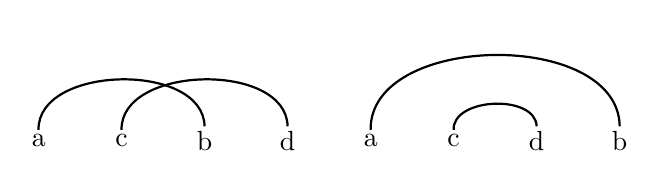
\begin{tikzpicture}
\node (a) {a};
\node [right of=a] (c) {c};
\node [right of=c] (b) {b};
\node [right of=b] (d) {d};

\drawedges[bend left,out=90,in=90]{a/b,c/d}

\begin{scope}[xshift=12em]
\node (a) {a};
\node [right of=a] (c) {c};
\node [right of=c] (d) {d};
\node [right of=d] (b) {b};

\drawedges[bend left,out=90,in=90]{a/b,c/d}
\end{scope}
\end{tikzpicture}
\end{figure}

Mirror image and cyclic shifts of a valid order remain valid:

\begin{figure}[\placement]
\centering

\resizebox{\textwidth}{!}{%
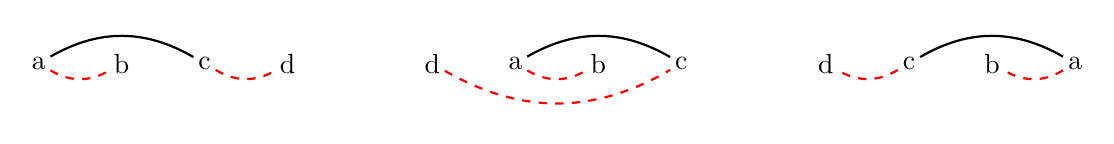
\begin{tikzpicture}
\begin{scope}
\node (a) {a};
\node [right of=a] (b) {b};
\node [right of=b] (c) {c};
\node [right of=c] (d) {d};

\draw (a) edge [bend left] (c);

\draw[edge1] (a) edge [bend right] (b);
\draw[edge1] (c) edge [bend right] (d);
\end{scope}

\begin{scope}[xshift=5cm]
\node (d) {d};
\node [right of=d] (a) {a};
\node [right of=a] (b) {b};
\node [right of=b] (c) {c};

\draw (a) edge [bend left] (c);
\draw[edge1] (a) edge [bend right] (b);
\draw[edge1] (d) edge [bend right] (c);
\end{scope}

\begin{scope}[xshift=10cm]
\node (d) {d};
\node [right of=d] (c) {c};
\node [right of=c] (b) {b};
\node [right of=b] (a) {a};

\draw (a) edge [bend right] (c);

\draw[edge1] (a) edge [bend left] (b);
\draw[edge1] (c) edge [bend left] (d);

\end{scope}
\end{tikzpicture}}
\end{figure}
\end{frame}

\resultFrame{1}

\begin{frame}
\frametitle{Contents}
\tableofcontents
\end{frame}

\miniframeson

%\section{Basic observations}

\begin{frame}{Total order formulation}
  Book embedding instance is solvable if and only if\\there is a total order~$<$ on~$V$ (\emph{valid order})
  without suborder \[a < c < b < d\] 
  for $\{a, b\}, \{c, d\} \in E_i$ (\emph{book constraint}).

\begin{figure}[\placement]
\centering

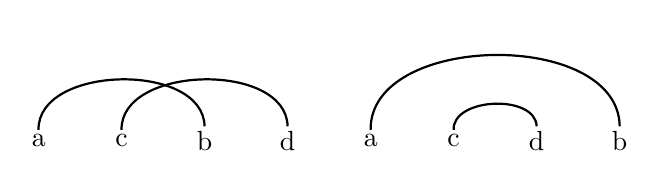
\begin{tikzpicture}
\node (a) {a};
\node [right of=a] (c) {c};
\node [right of=c] (b) {b};
\node [right of=b] (d) {d};

\drawedges[bend left,out=90,in=90]{a/b,c/d}

\begin{scope}[xshift=12em]
\node (a) {a};
\node [right of=a] (c) {c};
\node [right of=c] (d) {d};
\node [right of=d] (b) {b};

\drawedges[bend left,out=90,in=90]{a/b,c/d}
\end{scope}
\end{tikzpicture}

\end{figure}
\end{frame}

\begin{frame}{Valid orders}

Mirror image and cyclic shifts of valid order are valid:

\begin{figure}[\placement]
\centering

\resizebox{\textwidth}{!}{%
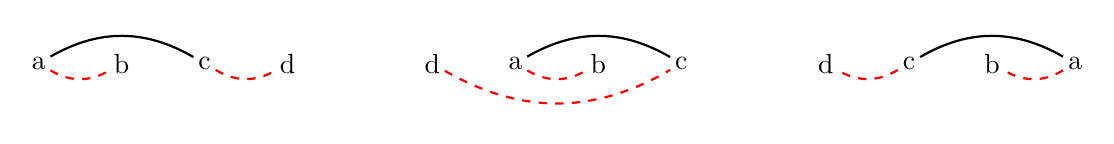
\begin{tikzpicture}
\begin{scope}
\node (a) {a};
\node [right of=a] (b) {b};
\node [right of=b] (c) {c};
\node [right of=c] (d) {d};

\draw (a) edge [bend left] (c);

\draw[edge1] (a) edge [bend right] (b);
\draw[edge1] (c) edge [bend right] (d);
\end{scope}

\begin{scope}[xshift=5cm]
\node (d) {d};
\node [right of=d] (a) {a};
\node [right of=a] (b) {b};
\node [right of=b] (c) {c};

\draw (a) edge [bend left] (c);
\draw[edge1] (a) edge [bend right] (b);
\draw[edge1] (d) edge [bend right] (c);
\end{scope}

\begin{scope}[xshift=10cm]
\node (d) {d};
\node [right of=d] (c) {c};
\node [right of=c] (b) {b};
\node [right of=b] (a) {a};

\draw (a) edge [bend right] (c);

\draw[edge1] (a) edge [bend left] (b);
\draw[edge1] (c) edge [bend left] (d);

\end{scope}
\end{tikzpicture}}

\end{figure}
\end{frame}

\section{\NP-completeness and connected pages}

\begin{frame}{\probBook is \NP-complete}

\begin{theorem}
\probBook with matchings as pages is \NP-complete.
\end{theorem}

Reduce from \NP-complete problem \probBetween [Opatrny, 1979].
\newProb{\probBetween}{Finite set $M := \range{n}$ and ordered triples $C \subseteq M^3$.}
{Is there a total ordering $<$ of $M$ such that $a < b < c$ or $a > b > c$ for all $(a, b, c) \in C$?}
\end{frame}

\begin{frame}{Reduction from \probBetween}

\newProb{\probBetween}{Finite set $M := \range{n}$ and ordered triples $C \subseteq M^3$.}
{Is there a total ordering $<$ of $M$ such that $a < b < c$ or $a > b > c$ for all $(a, b, c) \in C$?}

Map triple~$(a, b, c) \in C$ to two new pages ($r$ fixed new vertex):	
\begin{figure}
\centering

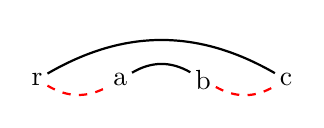
\begin{tikzpicture}
% a < b < c
\node (r) {r};
\node [right of=r] (a) {a};
\node [right of=a] (b) {b};
\node [right of=b] (c) {c};

\draw[edge1] (r) edge [bend right] (a);
\draw[edge1] (b) edge [bend right] (c);
\draw (a) edge [bend left]  (b);
\draw (r) edge [bend left]  (c);  
\end{tikzpicture}

\end{figure}

\begin{overprint}
\onslide<1>
For example: $(a, b, c)$, $(b, c, d)$
\begin{figure}\centering
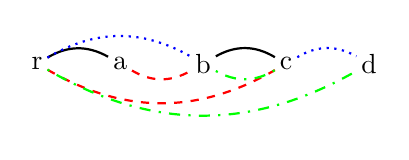
\begin{tikzpicture}
% a < b < c
\node (r) {r};
\node [right of=r] (a) {a};
\node [right of=a] (b) {b};
\node [right of=b] (c) {c};
\node [right of=c] (d) {d};

\drawedges[bend left]{r/a,b/c};
\drawedges[bend left,edge2]{r/b,c/d};
\drawedges[bend right,edge1]{a/b,r/c};
\drawedges[bend right,edge3]{b/c,r/d};
\end{tikzpicture}
\end{figure}

\onslide<2>
\probBetween $\Rightarrow$ \probBook:\\
Take~$r$ as first vertex\\
$\rightsquigarrow$ Orders $r < a < b < c$ or $r < c < b < a$ are valid

\onslide<3>
\probBook $\Rightarrow$ \probBetween:\\
Rotate $r$ to front\\
$\rightsquigarrow$ $r < a < b < c$ or $r < c < b < a$ are the only valid orders

\end{overprint}
\end{frame}



\begin{frame}<1>[label=connected,fragile]{Connected pages}

\begin{theorem}
\probBook with connected pages can be solved in $\OO(kn)$~time.
\end{theorem}

\begin{overprint}
\onslide<1>
Idea:\\Compute valid orders $\pi_i \subseteq \Sym(n)$ for single pages and\\intersect them.

\begin{figure}\centering
\resizebox{0.3\textwidth}{!}{
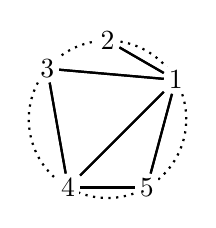
\begin{tikzpicture}
    \tikzstyle{every node}+=[fill=white]
	\draw[dotted] (0, 0) circle (1);
	\node (1) at (30:1) {1};
    \node (2) at (90:1) {2};
	\node (3) at (140:1) {3};
	\node (4) at (240:1) {4};
	\node (5) at (300:1) {5};
	\drawedges{1/2,3/4,1/3,1/4,1/5,4/5};
	\draw (1) -- (2);
	\draw (3) -- (4);
	\draw (1) -- (3);
	\draw (1) -- (4);
	\draw (1) -- (5);
	\draw (4) -- (5);
\end{tikzpicture}
}
\end{figure}

\onslide<2>

\begin{itemize}
\item Construct \PQ-trees $T_i$ on~$V$ representing valid orders of individual pages
$(V,E_i)$\hfill$\OO(n)$
\begin{figure}
\centering
\resizebox{0.6\textwidth}{!}{
\begin{tikzpicture}
\path[use as bounding box] (-2,2) rectangle (8,-2.5);

\tikzstyle{every node}+=[minimum size=0.5cm,thick]
\tikzstyle{every path}+=[thick]

\node[] (a) {$a$};
\node[right of=a] (b) {$b$};
\node[below of=b] (c) {$c$};
\node[left of=c] (d) {$d$};
\node[left of=a, above of=a] (r) {$r$};

\draw (a) edge (b) 
      (b) edge (c) 
      (c) edge (d) 
      (d) edge (a);
\draw[dashed] (r) edge (a)
              (r) edge (b)
              (r) edge (d)
              (r) edge[out=270, in=270, min distance=6em] (c);

% PQ-tree
\begin{scope}[xshift=5cm]
\node[draw,rectangle,minimum size=.2cm] {}
   child {node {$a$}}
   child {node {$b$}}
   child {node {$c$}}
   child {node {$d$}};
\end{scope}
\end{tikzpicture}}
\end{figure}

[Booth and Lueker et. al. 1976, Shih and Hsu 1993,\\Boyer and Myrvold 1999]
\end{itemize}

\onslide<3>
\begin{itemize}
\item Construct \PQ-trees $T_i$ on~$V$ representing valid orders of individual pages
$(V,E_i)$\hfill$\OO(n)$
\item Intersect the $T_i$ [Booth, 1975]\hfill$\OO(n)$
\item[$\rightarrow$] Resulting \PQ-tree~$T$ represents valid book orders
\end{itemize}
\end{overprint}

\end{frame} 

\begin{frame}{Interludium: \PQ-trees}

\begin{overprint}
\onslide<1>
$\hspace{4em}T = 
\begin{aligned}
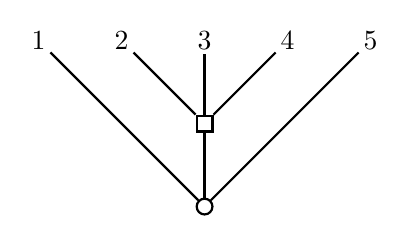
\begin{tikzpicture}

\tikzstyle{every path}+=[thick]

\node (1) {1};
\node[right of=1] (2) {2};
\node[right of=2] (3) {3};
\node[right of=3] (4) {4};
\node[right of=4] (5) {5};

\node[rectangle, draw, below of=3] (t2) {};
\node[circle, draw, below of=t2] (t1) {};

\draw (t1) edge (1);
\draw (t1) edge (5);
\draw (t2) edge (2);
\draw (t2) edge (3);
\draw (t2) edge (4);
\draw (t1) edge (t2);
\end{tikzpicture}
\end{aligned}$

\onslide<2>
$\hspace{4em}T = 
\begin{aligned}
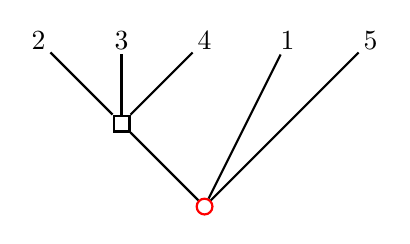
\begin{tikzpicture}

\tikzstyle{every path}+=[thick]

\node (2) {2};
\node[right of=2] (3) {3};
\node[right of=3] (4) {4};
\node[right of=4] (1) {1};
\node[right of=1] (5) {5};

\node[rectangle, draw, below of=3] (t2) {};
\node[circle, draw, below of=t2,right of=t2,red] (t1) {};

\draw (t1) edge (1);
\draw (t1) edge (5);
\draw (t2) edge (2);
\draw (t2) edge (3);
\draw (t2) edge (4);
\draw (t1) edge (t2);
\end{tikzpicture}
\end{aligned}$

\onslide<3>
$\hspace{4em}T = 
\begin{aligned}
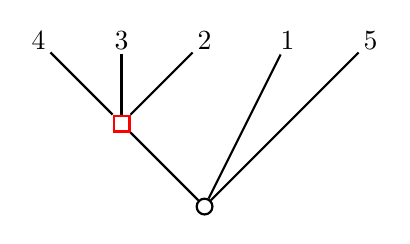
\begin{tikzpicture}

\tikzstyle{every path}+=[thick]

\node (4) {4};
\node[right of=4] (3) {3};
\node[right of=3] (2) {2};
\node[right of=2] (1) {1};
\node[right of=1] (5) {5};

\node[rectangle, draw, below of=3,red] (t2) {};
\node[circle, draw, below of=t2,right of=t2] (t1) {};

\draw (t1) edge (1);
\draw (t1) edge (5);
\draw (t2) edge (2);
\draw (t2) edge (3);
\draw (t2) edge (4);
\draw (t1) edge (t2);
\end{tikzpicture}
\end{aligned}$

\onslide<4>
$\hspace{4em}T = 
\begin{aligned}
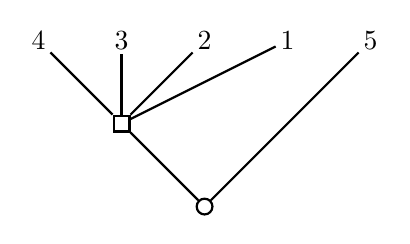
\begin{tikzpicture}

\tikzstyle{every path}+=[thick]

\node (4) {4};
\node[right of=4] (3) {3};
\node[right of=3] (2) {2};
\node[right of=2] (1) {1};
\node[right of=1] (5) {5};

\node[rectangle, draw, below of=3] (t2) {};
\node[circle, draw, below of=t2,right of=t2] (t1) {};

\draw (t2) edge (1);
\draw (t1) edge (5);
\draw (t2) edge (2);
\draw (t2) edge (3);
\draw (t2) edge (4);
\draw (t1) edge (t2);
\end{tikzpicture}
\end{aligned}$
\end{overprint}


\begin{overprint}
\onslide<1-3>
\begin{align*}
\pi(T) & = \{\only<1>{\alert{12345}}\only<2->{12345}, 14325, 52341, 54321, 15234, 15432, \\
         & \hspace{1.8em} 51234, 51432, \only<2>{\alert{23415}}\only<1,3->{23415}, \only<3>{\alert{43215}}\only<1-2>{43215}, 23451, 43251\}
\end{align*}

\onslide<4>
\begin{align*}
\pi(T) & = \{\alert{12345}, 14325, 52341, \alert{54321}, 15234, 15432, \\
         & \hspace{1.8em} \alert{51234}, 51432, 23415, \alert{43215}, 23451, 43251\}
\end{align*}
Permutations with the leaves in $\{1, 2\}$ adjacent
\end{overprint}
\end{frame}

\againframe{connected}

\resultFrame{3}
%\section{Connected pages}

\begin{frame}[fragile]{Linear-time decision}

\begin{theorem}
\probBook with connected pages can be solved in $\OO(n)$~time.
\end{theorem}

\begin{overprint}
\onslide<1>
\begin{itemize}
\item Construct \PQ-trees $T_i$ on~$V$ representing valid orders of individual pages
$(V,E_i)$
\begin{figure}
\centering
\resizebox{0.8\textwidth}{!}{
\begin{tikzpicture}
\path[use as bounding box] (-2,2) rectangle (8,-2.5);

\tikzstyle{every node}+=[minimum size=0.5cm,thick]
\tikzstyle{every path}+=[thick]

\node[] (a) {$a$};
\node[right of=a] (b) {$b$};
\node[below of=b] (c) {$c$};
\node[left of=c] (d) {$d$};

\draw (a) edge (b) 
      (b) edge (c) 
      (c) edge (d) 
      (d) edge (a);
\end{tikzpicture}}
\end{figure}
\end{itemize}

\onslide<2>

\begin{itemize}
\item Construct \PQ-trees $T_i$ on~$V$ representing valid orders of individual pages
$(V,E_i)$
\begin{figure}
\centering
\resizebox{0.8\textwidth}{!}{
\begin{tikzpicture}
\path[use as bounding box] (-2,2) rectangle (8,-2.5);

\tikzstyle{every node}+=[minimum size=0.5cm,thick]
\tikzstyle{every path}+=[thick]

\node[] (a) {$a$};
\node[right of=a] (b) {$b$};
\node[below of=b] (c) {$c$};
\node[left of=c] (d) {$d$};
\node[left of=a, above of=a] (r) {$r$};

\draw (a) edge (b) 
      (b) edge (c) 
      (c) edge (d) 
      (d) edge (a);
\draw[dashed] (r) edge (a)
              (r) edge (b)
              (r) edge (d)
              (r) edge[out=270, in=270, min distance=6em] (c);

% PQ-tree
\begin{scope}[xshift=5cm]
\node[draw,rectangle,minimum size=.2cm] {}
   child {node {$a$}}
   child {node {$b$}}
   child {node {$c$}}
   child {node {$d$}};
\end{scope}
\end{tikzpicture}}
\end{figure}
\end{itemize}

\onslide<3>
\begin{itemize}
\item Construct \PQ-trees $T_i$ on~$V$ representing valid orders of individual pages
$(V,E_i)$
\item Intersect the $T_i$ [Booth, 1975]
\item[$\rightarrow$] Resulting \PQ-tree~$T$ represents valid book orders
\end{itemize}
\end{overprint}

\end{frame}

\section{Perfect Matchings}\label{section:matchings}

A diametrically opposed simplification to \myref{section:connected} is to take disjoint
perfect matchings as graphs on the pages since matchings are---in a sense---the most disconnected graphs apart
from isolated vertices.
That is, we least expect to be able to adapt the result for connected graphs to this new setting.
Note that this is only possible for an even number of vertices and remember that we
have shown the \NP-completeness when taking (not necessarily perfect) matchings as pages in \myref{section:np-complete}.

\newProb{\probMatching}
{Disjoint perfect matchings $E_1,\dotsc, E_k$ on a vertex
set $V$.}{Is there a book embedding of $(V, E_1),\dotsc, (V, E_k)$?}

In this section we first show that an embeddable instance of \probMatching has to be
\emph{bipartite}, \ie the \emph{union graph}~$(V, E_1\cup\dotsb\cup E_k)$ must be bipartite. Then we prove that the problem does not become trivial for any number~$k$ of pages
by providing positive and negative bipartite instances.
For all~$k$ we get a partition of $K_{k,k}$, the complete bipartite graph with $k$~left and $k$~right vertices, as smallest (vertex-minimal) positive bipartite instance and
for $k > 3$ we get another partition of~$K_{k,k}$ as smallest negative bipartite instance.
We show this by hand in \myref{subsec:four}. Getting a smallest bipartite counterexample
for~$k = 3$ is significantly more difficult and we have to resort to using computer assistance in
\myref{subsec:three}. Even with the computer we only manage to find a smallest
bipartite counterexample when two of the matchings are required to form a cycle.

\begin{figure}[\placement]\centering
    \includegraphics[scale=2.0]{figures/t_k4}
    \caption[$K_4$ is not embeddable]{A non-embeddable partition of $K_4$.}
    \label{figure:k4}
\end{figure}

The partition of $K_4$, the complete graph on four~vertices, depicted in \myref{figure:k4} is already a counterexample to \probMatching with three pages.
This can be checked by hand or by using the corresponding \probThreeSat instance we derived
in \myref{section:sat}. We observe that the main reason for its non-embeddability is
the non-bipartiteness of~$K_4$ since bipartiteness is necessary for embeddability,
as we prove in the following theorem.

\begin{figure}\centering
    \includegraphics{figures/t_bipartite}
    \caption[Embeddable perfect matchings have to be bipartite]{There is an even number of vertices between $v$ and each neighbour $n_i(v)$.}
    \label{figure:bipartite}
\end{figure}

\begin{theorem}
\label{lemma:bipartite}
Let $I := (V, E_1,\dotsc, E_k)$ be an instance of \probMatching. If the graph
$G := (V, E_1 \cup \dotsb \cup E_k)$ is not bipartite, it has no book embedding.
\end{theorem}
\begin{myproof}
Assume we have a valid book order~$<$ for $G$ and let~$s(v)$ be the index of~$v \in V$,
\ie $s(v) = j$ if and only if~$v$ is the $j$-th smallest element in~$<$. We show that~$G$
is bipartite with the bipartitions given by the parity of the index of a vertex,
\ie $V_E := \bigl\{v \in V\colon \text{$s(v)$ is even}\bigr\}$ and $V_O := V \setminus V_E = \bigl\{v \in V\colon \text{$s(v)$ is odd}\bigr\}$ is a bipartition of~$G$.

Let $i \in \range{k}$.
Every vertex~$v\in V$ is incident to exactly one edge in each set~$E_i$. 
We can, therefore, define~$n_i(v)$ to be the unique neighbour of~$v$ in the graph~$(V, E_i)$.
The neighbour~$n_i(w)$ of a vertex~$w$ between~$n_i(v)$ and~$v$ in the order~$<$ has to
occur between~$n_i(v)$ and~$v$ since~$<$ fulfils the book constraints. That is,
the vertices between~$n_i(v)$ and~$v$ appear in pairs. There is, therefore, an even number 
of vertices between~$n_i(v)$ and~$v$, as depicted in \myref{figure:bipartite}, and the index of~$n_i(v)$ has a different parity than the index of~$v$.

We conclude that~$(V_O, V_E)$ is indeed a bipartition of~$G$ and bipartiteness is, therefore, necessary
for book embeddability.
\end{myproof}

\begin{subsection}{Bipartite Examples with at Least Four~Pages}\label{subsec:four}

We know that non-bipartite graphs are not embeddable. But are there also bipartite counterexamples
for all number of pages, or is the problem the same as testing bipartiteness? (That would be surprising since the slightly more general problem \probNotMatching is \NP-complete for a linear number of pages.) 

At the other extreme, we ask whether there are positive instances
for all number of pages. The number of edges
in the whole graph is $(nk)/2$ for~$n$ vertices and $k$~pages. That is, 
approximately~$k/n$ of the possible edges are present. Therefore,
the resulting graph cannot be too small and it is not immediately apparent that there
are positive bipartite instances for large~$k$.

\begin{figure}\centering
    \includegraphics[width=\textwidth]{figures/t_two_matchings}
    \caption[One and two matchings]{One matching just consists of independent edges, while two matchings form disjoint cycles.}
    \label{figure:two_matchings}
\end{figure}

For one~matching, $G$~is a perfect matching which is obviously embeddable.
For two~matchings, every vertex of~$G$ has degree~2, \ie $G$ consists of disjoint
even cycles. Thus, $G$~is embeddable by placing the vertices of the cycles consecutively.
These cases are illustrated in \myref{figure:two_matchings}.

We now consider the larger cases.
Our goal is to provide both positive and negative
bipartite instances for \probMatching and all $k \geq 3$.

In this subsection we give examples for all $k \geq 4$ and
prove their embeddability or non-embeddability, respectively, by hand.
We believe that these proofs are vastly more illuminating than
just using a \SAT solver as a black-box. For the significantly more
difficult case~$k = 3$ we use computer assistance in the following subsection.

Surprisingly, the smallest bipartite graph~$K_{k,k}$ that can be split
into~$k$ perfect matchings provides us with both a positive and
a negative instance; but we still have to choose the perfect matchings sensibly.

Consider the partition of $K_{4,4}$ of \myref{figure:split_k4}.
It was chosen such that any two matchings form two cycles of length 4. We prove
that this partition is not embeddable.

\begin{figure}[\placement]\centering
    \includegraphics{figures/t_split_k4}
    \caption[$K_{4,4}$ has a non-embeddable partition]{A non-embeddable partition of $K_{4,4}$.}
    \label{figure:split_k4}
\end{figure}

\begin{lemma}
\label{lemma:split_k4}
The partition of~$K_{4,4}$ given in \myref{figure:split_k4} is not book
embeddable.
\end{lemma}
\begin{myproof}
We are looking for a valid book order~$<$. From the proof of \myref{lemma:bipartite}
we get that the left and right vertices have positions of different parity under~$<$.
Let~$v_i$ be the $i$-th smallest vertex under~$<$ for $i \in \range{8}$. Then $v_1$ is adjacent to $v_2$ and $v_2$ is adjacent to $v_3$ since our graph is $K_{4,4}$ .

For reasons of symmetry, we can, therefore, assume $v_1 = l_1$, $v_2 = r_1$ and $v_3 = l_2$.
By~\myref{lemma:np-c4} this fixes the order of the vertices of both the black/blue~(solid/dotted)~$C_4$ containing~$l_1$ and the black/green~(solid/dash-dotted)~$C_4$ containing~$r_1$, \ie $l_1 < r_1 < l_3 < r_3$ and $l_1 < r_1 < l_4 < r_4$.
Since the left and the right vertices alternate, the black/red~(solid/dashed) $C_4$ formed by $\{l_3, r_3, l_4, r_4\}$ now yields $l_3 < r_3 < l_4 < r_4$ or $l_4 < r_4 < l_3 < r_3$. Assume $l_3 < r_3 < l_4 < r_4$
in the following. The other case can be handled analogously. 

\begin{figure}[\placement]\centering
    \includegraphics{figures/t_not_embeddable}
    \caption{Partial embedding of the partition in \myref{figure:split_k4}.}
    \label{figure:partial_k4}
\end{figure}

The partial embedding we have so far is depicted in \myref{figure:partial_k4}.	
We see that the blue (dotted) edge $l_2r_4$ intersects the blue (dotted) edge $r_1l_3$.
Thus, the graph is not book embeddable.

%The only vertex we still have to place is $r_2$. If $r_2$ were not between $l_2$ and $l_3$, then
%the red edge $l_1r_2$ would intersect with another red edge. But if $l_2 < r_2 < l_3$, then
%$l_2r_4$ intersects with $r_2l_4$. 
\end{myproof}

We can build partitions of $K_{k,k}$ into
disjoint perfect matchings that contain the non-embeddable partition of~$K_{4,4}$. These partitions
of~$K_{k,k}$ are then obviously also not embeddable.

The positive instance we are looking for is somewhat harder to find since a graph
containing a positive instance does not itself have to be book embeddable. That is, we have to
explicitly give an embedding for every $k \geq 4$ and cannot just prove that some
graph with $k=4$ is embeddable and extend it to a partition of~$K_{k,k}$ for larger~$k$.

We label the left vertices with~$\{l_0,\dotsc, l_{k-1}\}$ and the right vertices with~$\{r_0,\dotsc, r_{k-1}\}$.
It then turns out that the \emph{cyclic partition} $E_i := \bigl\{\{l_j, r_{(j + i)\mymod{k}}\}: j \in \range{k-1}\bigr\}$ into matchings is embeddable.
The case~$k=4$ is illustrated in \myref{figure:cycle_k4}. 

\begin{figure}[\placement]\centering
    \includegraphics[scale=2.0]{figures/t_cycle_k4}
    \caption[$K_{4,4}$ has an embeddable partition]{The cyclic partition of $K_{4,4}$ is embeddable.}
    \label{figure:cycle_k4}
\end{figure}

\begin{lemma}
The complete bipartite graph $K_{k,k}$ with the cyclic partition is
book embeddable.
\end{lemma}
\begin{myproof}
We get a valid order of the vertices by alternatingly listing the right vertices
in increasing order and the left vertices in decreasing:
\[
r_0 < l_{k-1} < r_1 < l_{k-2} < \dotsb < r_{k-1} < l_0\tag{1}
\]
In the first matching~$E_0$
the first vertex~$r_0$ is matched with the last vertex~$l_0$, the
second vertex~$l_{k-1}$ with the penultimate vertex~$r_{k-1}$, and so on.
That is, the book constraints of \myref{lemma:constraints} are fulfilled for the page~$E_0$ in the order~(1). More specifically,
we get concentric semi-circles as canonical embedding in the proof of \myref{lemma:constraints}.

Now let~$i \in \range{k-1}$ and consider the matching~$E_i$. Both~$E_i$ and~$E_0$ are perfect matchings on the vertices of~$K_{k, k}$, \ie they are isomorphic.
Still, $E_i$ is somewhat harder to understand since it is shifted. To simplify the matching~$E_i$
we now want to relabel the right vertices~$r_j$ such that~$E_i$ matches $l_j$ to~$r_j$
for each~$j\in\{0, \dotsc, k-1\}$.  We achieve this by renaming $r_i, \dotsc, r_{k-1}$
to~$r_0, \dotsc, r_{k-i-1}$ as well as $r_0, \dotsc, r_{i-1}$ to~$r_{k-i}, \dotsc, r_{k-1}$ in this order.

After applying this relabelling to the original order, we get
\[
r_{k-i} < l_{k-1} < \dotsb < r_{k-1} < l_{k-i} < r_0 < l_{k-i-1} < \dotsb < r_{k-i-1} < l_0.\tag{2}
\]
Since $E_i$ now matches each $l_j$ to~$r_j$, we see that 
when we cut the vertices between $l_{k-i}$ and~$r_0$,
we get two independent sets of concentric semi-circles as canonical embedding (\myref{lemma:constraints}) of~$E_i$ in the order~(2) which the same as the order~(1) after a change of name. Thus, the book constraints are fulfilled for the page~$E_i$.\qedhere

%By construction of the order we get
%\begin{align}
%l_i < r_j & \Leftrightarrow i + j < n, \tag{1}\\
%l_i < l_j & \Leftrightarrow i > j, \tag{2}\\
%r_i < r_j & \Leftrightarrow i < j \tag{3}
%\end{align}
%for all~$i, j \in \range{n-1}$.
%
%Now take two edges $e_1 := \{i, j\}$ and $e_2 := \{k, s\}$ from the same matching and
%show the book constraint for them. 
%
%We only consider the case $i < j$ and $k < s$ since
%the other cases are symmetric. As $e_1$ and~$e_2$ are in the same matching,
%$j - i = s - k$~(4) has to hold.
%
%We may again only consider one of the symmetric cases for
%the book constraints: Assume $l_i < r_s < r_j$ and show $l_i < l_k < r_j$.
%
%The assumption $l_i < r_s < r_j$ along with the observations (1) and (3) yields $i + s < n$ and~$s < j$, respectively. With (4) we can infer $k + j = i + s < n$, \ie $l_k < r_j$ by (1).
%Similarly, $k = s - j + i < j - j + i = i$ and, therefore, (2)~implies $l_i < l_k$. 
%
%So the order given above is indeed valid.
\end{myproof}
%\begin{figure}[\placement]
\centering

\begin{tikzpicture}
\node (r0) {$r_0$};
\node[right of=r0] (lnm) {$l_{n-1}$};
\node[right of=r1] (p) {$\dots$};
\node[right of=p] (rnmmm) {$r_{n - 3}$};
\node[right of=rnmmm] (l2) {$l_2$};
\node[right of=l2] (rnmm) {$r_{n - 2}$};
\node[right of=rnmm] (l1) {$l_1$};
\node[right of=l1] (rnm) {$r_{n - 1}$};
\node[right of=rnm] (l0) {$l_0$};

\semicircle{r0}{l2};
\semicircle{lnm}{rnmmm};
\semicircle{rnmm}{l1};
\semicircle{rnm}{l0};

\end{tikzpicture}

\label{figure:cycle_k4_proof}
\caption[Cyclic embedding has concentric semi-circles]{The embedding for the cyclic partition consists of sets of concentric semi-circles
for each matching. The matching $E_2$ is drawn.}
\end{figure}


\end{subsection}

\subsection{Bipartite Counterexamples with Three Matchings}\label{subsec:three}

As alluded to above, in this subsection we determine a smallest bipartite counterexample for
three disjoint perfect matchings when two of the matchings form a cycle. 

We first give the case with three pages a name.

\newProb{\probThreeMatching}
{Three disjoint perfect matchings $E_1$, $E_2$ and $E_3$ on a vertex
set $V$.}{Is there a book embedding of $(V, E_1)$, $(V, E_2)$, $(V, E_3)$?}

The smallest possible \probThreeMatching instance~$K_4$ is already a non-bipartite counterexample,
as shown at the start of this section. In contrast,
we do not immediately see a bipartite counterexample. In fact, the smallest bipartite counterexample
has at least 20~vertices, as we see below. It can, therefore, not be viably found without computer assistance.
In this subsection we describe how we used the computer to do so.

We already know from \myref{section:sat} how a single book embedding instance can be tested using a \SAT-solver. To look for a counterexample, we, naturally, just iterate over all bipartite instances of~\probMatching in increasing (even) order and test them for book embeddability.

\begin{figure}[\placement]
    \centering
    \includegraphics{figures/t_bip_cycle}
    \caption[One cycle consisting of two matchings]{Two matchings form a cycle.}
    \label{figure:bip_cycle}
\end{figure}
    
This has to be done somewhat intelligently, using the symmetries of the problem, to remain
in reasonable time. One improvement we use is to utilise multiple cores
by letting the instance generator and the \SAT-solvers run in parallel. How the
solver stage can be accelerated by optimising the \SAT-formulae was already discussed in \myref{section:sat}. Below we show
how to optimise the actual generator. 

Even so, it is still too slow to get the
smallest bipartite counterexample with the available computing hardware ($4\times12$-Core AMD Opteron 6172, 2.1 GHz, 256 GB RAM). Therefore, we first
provide the smallest counterexample for an even more restricted instance, namely that two of the matchings
form a single cycle. It has order~28. We then proceed with the general \probThreeMatching problem
and compute that there is no bipartite counterexample with~$\leq \text{18}$ vertices.

\paragraph{Two matchings form a cycle}

At the start, we restrict ourselves to instances where two of the matchings 
form a cycle. Without loss of generality the cycle contains the vertices from~$0$ to~$n - 1$ in order, the first matching is $\bigl\{\{l, (l + 1)\mymod{n}\}\colon l \in \range{n-1}, \text{$l$ even}\bigr\}$ and
the second is $\bigl\{\{l, (l + 1)\mymod{n}\}\colon l \in \range{n-1}, \text{$l$ odd}\bigr\}$, as depicted in \myref{figure:bip_cycle}. This labelling already fixes the bipartition. The odd vertices
form the first partition and the even vertices the second. The third matching can then be filled
using backtracking by successively adding edges that do not already exist between vertices of different parity.

But there is another symmetry we can use, namely the rotational symmetry from \myref{lemma:symmetry}. For this reason, we first define a value for edges that is invariant under
cyclic shifts and can be interpreted as edge length in the corresponding symmetric order.

\begin{figure}[\placement]
    \centering
    \includegraphics{figures/t_bip_length}
    \caption[Cyclic length of an edge]{The value $\mu(v) = \min\{d_1, d_2\}$ is the length of the edge $\{v, w\}$ in the symmetric order.}
    \label{figure:bip_length}
\end{figure}
  
\begin{deflemma}
Let~$<$ be a total order on~$V := \{0, \dotsc, n-1\}$, $E$ a~matching and $v \in V$. Furthermore,
let~$w$ be the unique neighbour of $v$ in $E$ and $i: V \rightarrow V$ the index function of~$<$.

Then define~$\mu(v) := \min\bigl\{|i(v) - i(w)|, n - |i(v) - i(w)|\bigr\}$. The value~$\mu(v)$ is invariant
under cyclic shifts of~$<$.
\end{deflemma}
\begin{myproof}
If we consider the symmetric order~$[<]$ corresponding to~$<$, $\mu(v)$~can be interpreted as the length of
the edge $\{v, w\}$ as in \myref{figure:bip_length}. It is then clearly invariant 
under cyclic shifts.
\end{myproof}

We can, therefore, always rotate an instance such that the edge incident to~$0$ in the third
matching has the largest length~$\mu(\cdot)$. That is, we can first determine the edge incident to~$0$ in the backtracking
process and need only consider edges with length at most~$\mu(0)$ in the following backtracking steps.

Our implementation of this search strategy yields the graph in \myref{figure:two_cycles}
as one of the smallest counterexamples. In this example both the red/blue (dashed/dotted) pages
and the red/black (dashed/solid) pages form cycles.
There are other non-isomorphic bipartite counterexamples of this size that we do not depict.

Thus, a bipartite counterexample has at 
least~28 vertices in this special case. It may be possible
to infer a useful sufficient condition for \probThreeMatching from it. But
we were unable to do so since the depicted graph is quite large and asymmetric.

\begin{figure}[\placement]
\centering

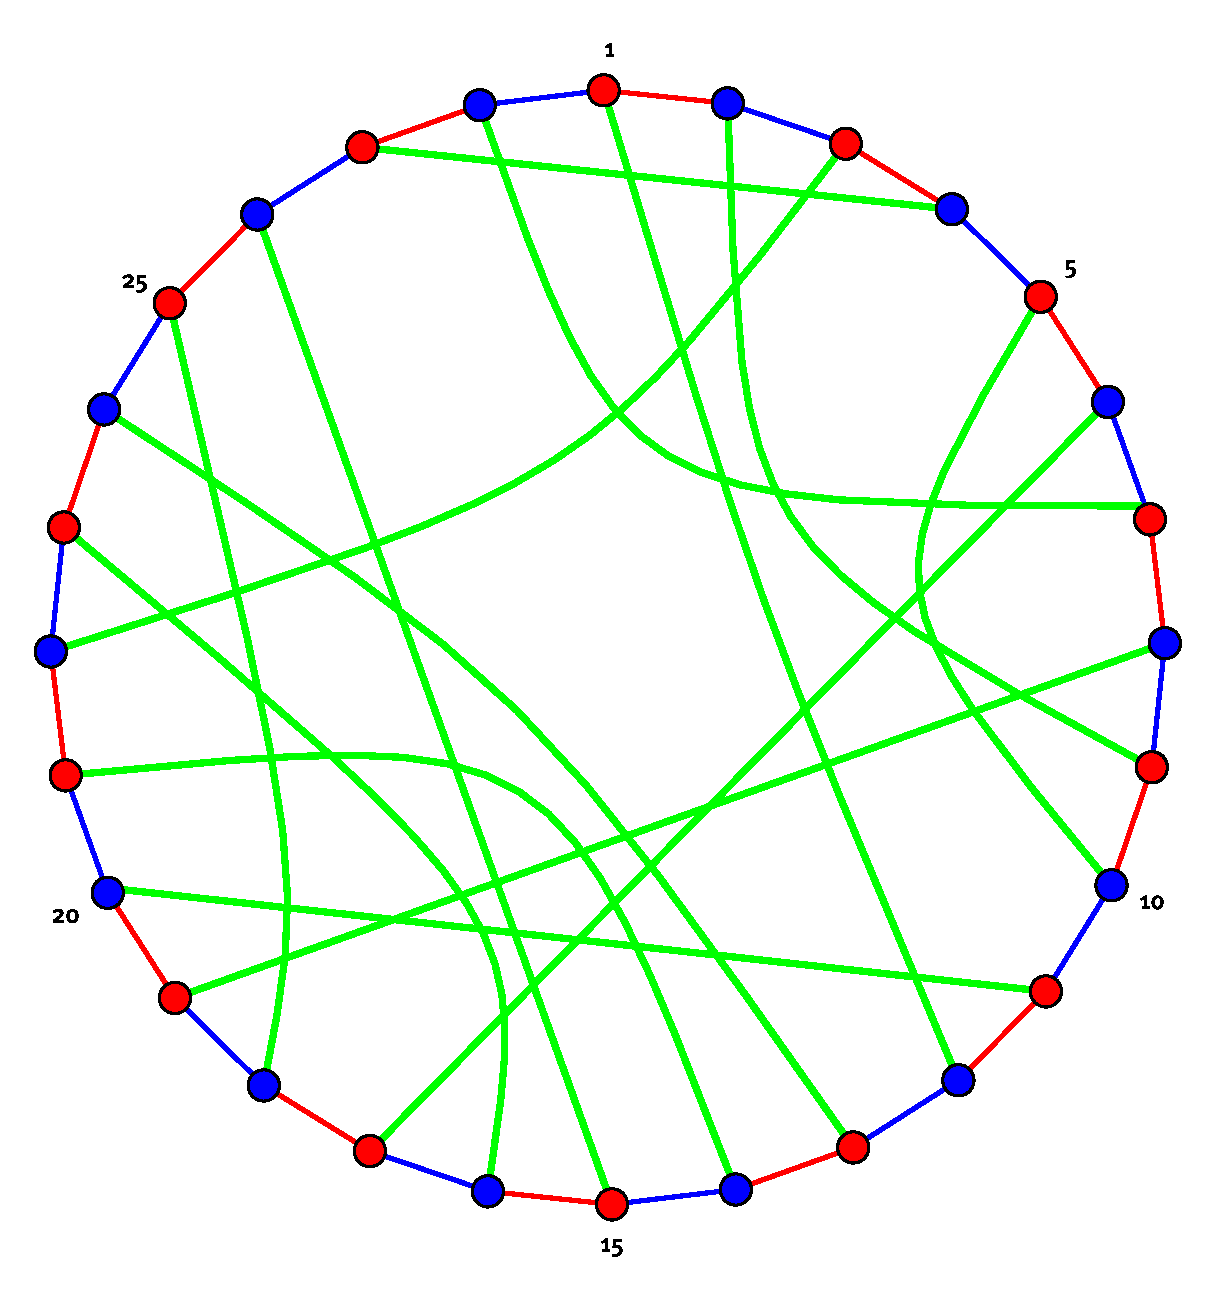
\includegraphics[width=0.95\textwidth]{figures/two_cycles.pdf}

\caption[Smallest bipartite counterexample with three pages]{Smallest bipartite counterexample with three pages containing perfect disjoint matchings where two of the matchings form a cycle.}
\label{figure:two_cycles}
\end{figure}

\paragraph{No restrictions}

If we abandon the restriction that two of the matchings form a cycle, we can proceed similarly. 
Without loss of generality the first matching connects every even vertex to the following odd
vertex. Then the odd and even vertices form the bipartition. The remaining two matchings
can then be filled in by backtracking and adding edges between vertices with different parity. By exchanging
the second and third matching and rotating we can again impose the restriction that~$\mu(0)$
in the second matching is the maximal value of~$\mu(\cdot)$ in both the second and the third matching.

The search space is significantly larger since we abandoned the restriction that two
matchings form a cycle. Thus, we were only able to check for counterexamples up to order~18, which already took a week on the available computing hardware ($4\times12$-Core AMD Opteron 6172, 2.1 GHz, 256 GB RAM). %For 20~vertices
%the program needed too long (TODO, ...). 

We did not find any counterexample with~$\leq 18$ vertices.
That is, we can only conclude that \probThreeMatching
has a smallest bipartite counterexample with at least 20~vertices and at most 28~vertices.

\paragraph{Outlook}

It is, therefore, a sensible extension of this work to implement a
more efficient searcher or just use more computing power to get the
smallest counterexample of \probThreeMatching. 

Also, the special case \probThreeMatching may already be \NP-complete.
It may be possible
to  disprove this by getting a simple decision criterion 
from the structure of the counterexample in \myref{figure:two_cycles}.
Inversely, the example may also provide a clue on how to prove the \NP-hardness. This
direction seems to be quite difficult since we do not really understand why this example is a counterexample.
\section{Tree on the vertices}

\begin{frame}{Tree on the vertices}

\probBook + tree:

\begin{overprint}
\onslide<1>
\begin{figure}\centering
\includegraphics[width=0.8\textwidth]{sefe2}
\end{figure}

Drawing the tree = Restricting permutations by a \PT-tree

\onslide<2>
\vspace{-1em}
\newProb{\probPTree}{\probBook instance $I$ and a \PT-tree~$T$ with leaves~$V$.}{Is there a total order $<\,\in \pi(T)$ solving $I$?}

More structure (same for binary trees):
\newProb{\probQTree}{\probBook instance $I$ and a \Q-tree~$T$ with leaves~$V$.}{Is there a total order $<\,\in \pi(T)$ solving $I$?}
\end{overprint}
\end{frame}

\begin{frame}{Example}

\begin{overprint}

\onslide<1>
\begin{figure}
\centering
\scalebox{1.0}{%
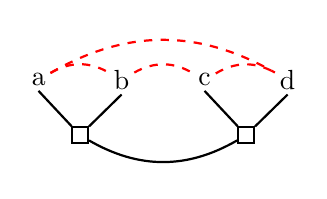
\begin{tikzpicture}
% ab || cd
\begin{scope}
\node (a) {a};
\node[right of=a] (b) {b};
\node[right of=b] (c) {c};
\node[right of=c] (d) {d};

\node[rectangle, draw] (c1) at ($ 0.5*($(a) + (b)$) + (0, -2em) $) {};
\node[rectangle, draw] (c2) at ($ 0.5*($(c) + (d)$) + (0, -2em) $) {};

\draw (c1) edge (a.south);
\draw (c1) edge (b.south);
\draw (c2) edge (c.south);
\draw (c2) edge (d.south);
\draw (c2) edge[bend left] (c1);
\end{scope}

\drawedges[bend left,edge1]{a/b,c/d}
\drawedges[bend left,edge1]{b/c,a/d}
\end{tikzpicture}}
\end{figure}

\begin{itemize}
  \item What happens to the forbidden suborder constraint?
  \item[$\Rightarrow$] 2-CNF formula (Boolean equations) on orientation of \Q-nodes
\end{itemize}

\onslide<2>
\begin{figure}
\centering
\scalebox{1.0}{%
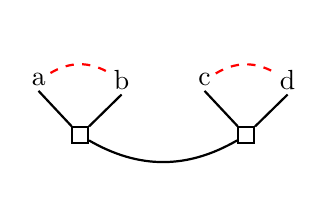
\begin{tikzpicture}
% ab || cd
\begin{scope}
\node (a) {a};
\node[right of=a] (b) {b};
\node[right of=b] (c) {c};
\node[right of=c] (d) {d};

\node[rectangle, draw] (c1) at ($ 0.5*($(a) + (b)$) + (0, -2em) $) {};
\node[rectangle, draw] (c2) at ($ 0.5*($(c) + (d)$) + (0, -2em) $) {};

\draw (c1) edge (a.south);
\draw (c1) edge (b.south);
\draw (c2) edge (c.south);
\draw (c2) edge (d.south);
\draw (c2) edge[bend left] (c1);
\end{scope}

\drawedges[bend left,white]{b/c,a/d}
\drawedges[bend left,edge1]{a/b,c/d}
\end{tikzpicture}}
\end{figure}

\begin{itemize}
\item $\{a, b\}$, $\{c, d\}$: \bool{true}
\end{itemize}
\onslide<3>

\begin{figure}
\centering
\scalebox{0.8}{%
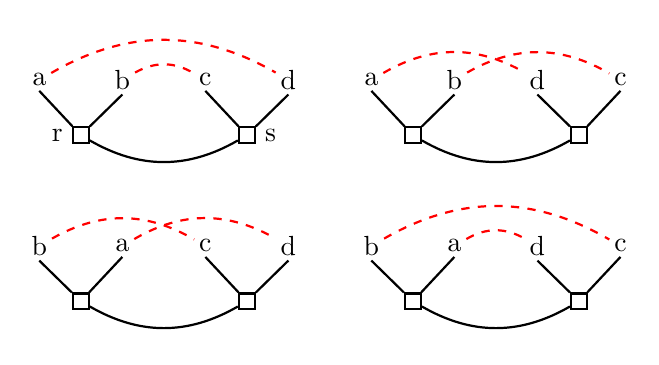
\begin{tikzpicture}
% ab || cd
\begin{scope}
\node (a) {a};
\node[right of=a] (b) {b};
\node[right of=b] (c) {c};
\node[right of=c] (d) {d};

\node[rectangle, draw] (c1) at ($ 0.5*($(a) + (b)$) + (0, -2em) $) {};
\node[rectangle, draw] (c2) at ($ 0.5*($(c) + (d)$) + (0, -2em) $) {};
\node at ($ (c1) + (-.3,0)$) {r};
\node at ($ (c2) + (+.3,0)$) {s};

\draw (c1) edge (a.south);
\draw (c1) edge (b.south);
\draw (c2) edge (c.south);
\draw (c2) edge (d.south);
\draw (c2) edge[bend left] (c1);
\drawedges[bend left,edge1]{b/c,a/d}
\end{scope}

\begin{scope}[xshift=12em]
\node (a) {a};
\node[right of=a] (b) {b};
\node[right of=b] (c) {d};
\node[right of=c] (d) {c};

\node[rectangle, draw] (c1) at ($ 0.5*($(a) + (b)$) + (0, -2em) $) {};
\node[rectangle, draw] (c2) at ($ 0.5*($(c) + (d)$) + (0, -2em) $) {};

\draw (c1) edge (a.south);
\draw (c1) edge (b.south);
\draw (c2) edge (c.south);
\draw (c2) edge (d.south);
\draw (c2) edge[bend left] (c1);
\drawedges[bend left,edge1]{b/d,a/c}
\end{scope}

\begin{scope}[yshift=-6em]
\node (a) {b};
\node[right of=a] (b) {a};
\node[right of=b] (c) {c};
\node[right of=c] (d) {d};

\node[rectangle, draw] (c1) at ($ 0.5*($(a) + (b)$) + (0, -2em) $) {};
\node[rectangle, draw] (c2) at ($ 0.5*($(c) + (d)$) + (0, -2em) $) {};

\draw (c1) edge (a.south);
\draw (c1) edge (b.south);
\draw (c2) edge (c.south);
\draw (c2) edge (d.south);
\draw (c2) edge[bend left] (c1);
\drawedges[bend left,edge1]{a/c,b/d}
\end{scope}

\begin{scope}[yshift=-6em,xshift=12em]
\node (a) {b};
\node[right of=a] (b) {a};
\node[right of=b] (c) {d};
\node[right of=c] (d) {c};

\node[rectangle, draw] (c1) at ($ 0.5*($(a) + (b)$) + (0, -2em) $) {};
\node[rectangle, draw] (c2) at ($ 0.5*($(c) + (d)$) + (0, -2em) $) {};

\draw (c1) edge (a.south);
\draw (c1) edge (b.south);
\draw (c2) edge (c.south);
\draw (c2) edge (d.south);
\draw (c2) edge[bend left] (c1);
\drawedges[bend left,edge1]{b/c,a/d}
\end{scope}

\end{tikzpicture}}
\end{figure}

\begin{itemize}
\item $\{a, d\}$, $\{b, c\}$: $a < b \Leftrightarrow c < d$\\
\item Fix reference orientation of inner nodes~$r$
\item Boolean variable~$o_r$ for being in reference orientation  
\item[$\Rightarrow$] $o_r \Leftrightarrow o_s$
\end{itemize}
\end{overprint}
\end{frame}

%\begin{frame}{Quadratic-time decision}
%%Idea:
%\begin{itemize}
%\item Map to \probTwoSat instance
%\item Fix reference orientation of inner nodes~$r$ of~$T$
%\item Let Boolean variable $o_r$ express~$r$ being in reference orientation
%\item Constraint for two edges yields 2-\CNF formula in constant time
%\end{itemize}
%\end{frame}

%\begin{frame}{Conventions}
%\begin{itemize}
%  \item Let $(V, E_1, \dotsc, E_k)$ be the \probBook instance we consider and $T$~be the \Q-tree on the leaves~$V$ that the vertex order should come from
%  \item For all~$M \subseteq V$ let $r(M)$ be the lowest common ancestor of the vertices~$M$ in~$T$
%  \item Fix a reference orientation for all inner nodes~$r$ of~$T$
%  \item Let the Boolean variable~$o_r$ express~$r$ being in reference orientation 
%\end{itemize}
%\end{frame}

%%%%%%%%%%%%%%%%%%%%%%%%% Book constraints
\begin{frame}{Book constraints to 2-\CNF formula}

\begin{theorem}
\probQTree is solvable in $\OO(kn^2)$ time.
\end{theorem}

\vspace{-.5em}
{
\begin{tabular}{m{0.2\textwidth}m{0.8\textwidth}}


%%% ROW 1
\begin{figure}
\centering
\resizebox{0.2\textwidth}{!}{%
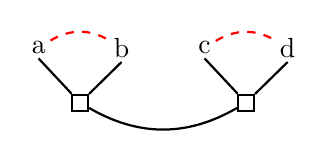
\begin{tikzpicture}
% ab || cd
\begin{scope}
\node (a) {a};
\node[right of=a] (b) {b};
\node[right of=b] (c) {c};
\node[right of=c] (d) {d};

\node[rectangle, draw] (c1) at ($ 0.5*($(a) + (b)$) + (0, -2em) $) {};
\node[rectangle, draw] (c2) at ($ 0.5*($(c) + (d)$) + (0, -2em) $) {};

\draw (c1) edge (a.south);
\draw (c1) edge (b.south);
\draw (c2) edge (c.south);
\draw (c2) edge (d.south);
\draw (c2) edge[bend left] (c1);
\end{scope}
\drawedges[bend left,edge1]{a/b,c/d}
\end{tikzpicture}}
\end{figure} &
\bool{true}\\[-2em]

%%% ROW 2
\begin{figure}
\centering

\resizebox{0.2\textwidth}{!}{%
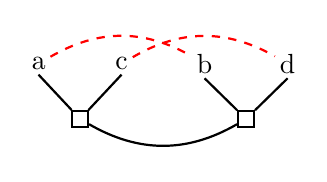
\begin{tikzpicture}

% ac || bd
\begin{scope}[xshift=5cm]
\node (a) {a};
\node[right of=a] (b) {c};
\node[right of=b] (c) {b};
\node[right of=c] (d) {d};

\node[rectangle, draw] (c1) at ($ 0.5*($(a) + (b)$) + (0, -2em) $) {};
\node[rectangle, draw] (c2) at ($ 0.5*($(c) + (d)$) + (0, -2em) $) {};

\draw (c1) edge (a.south);
\draw (c1) edge (b.south);
\draw (c2) edge (c.south);
\draw (c2) edge (d.south);
\draw (c2) edge[bend left] (c1);
\drawedges[bend left,edge1]{a/c,b/d}
\end{scope}

\end{tikzpicture}}
\end{figure}
 
 & \bool{o_{r(a, c)} \Leftrightarrow o_{r(b, d)}} or 
     \bool{o_{r(a, c)} \Leftrightarrow \lnot o_{r(b, d)}} \\[-2em]

%%% ROW 3
  \begin{figure}
  \centering

\resizebox{0.2\textwidth}{!}{%
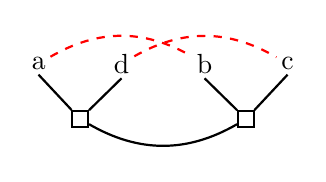
\begin{tikzpicture}
% ad || bc
\begin{scope}[xshift=0cm,yshift=-3cm]
\node (a) {a};
\node[right of=a] (b) {d};
\node[right of=b] (c) {b};
\node[right of=c] (d) {c};

\node[rectangle, draw] (c1) at ($ 0.5*($(a) + (b)$) + (0, -2em) $) {};
\node[rectangle, draw] (c2) at ($ 0.5*($(c) + (d)$) + (0, -2em) $) {};

\draw (c1) edge (a.south);
\draw (c1) edge (b.south);
\draw (c2) edge (c.south);
\draw (c2) edge (d.south);
\draw (c2) edge[bend left] (c1);
\drawedges[bend left,edge1]{a/c,b/d}
\end{scope}
\end{tikzpicture}}
\end{figure} &
     \bool{o_{r(a, d)} \Leftrightarrow o_{r(b, c)}} or
     \bool{o_{r(a, d)} \Leftrightarrow \lnot o_{r(b, c)}}\\[-1.5em]

%%% ROW 4
  \begin{figure}
\centering

\resizebox{0.2\textwidth}{!}{%
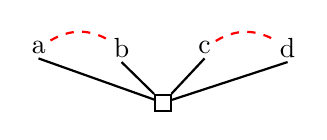
\begin{tikzpicture}
% abcd
\begin{scope}[xshift=5cm,yshift=-3cm]
\node (a) {a};
\node[right of=a] (b) {b};
\node[right of=b] (c) {c};
\node[right of=c] (d) {d};

\node[rectangle, draw] (c1) at ($ 0.5*($(b) + (c)$) + (0, -2em) $) {};

\draw (c1) edge (a.south);
\draw (c1) edge (b.south);
\draw (c1) edge (c.south);
\draw (c1) edge (d.south);
\drawedges[bend left,edge1]{a/b,c/d}
\end{scope}
\end{tikzpicture}} 
\end{figure} & \bool{true} or \bool{false}

\end{tabular}}
\end{frame}
%\section{Multiple spines}

\begin{frame}{Multiple spines}
Take multiple spines:
\tikzsetnextfilename{t_two_spines}
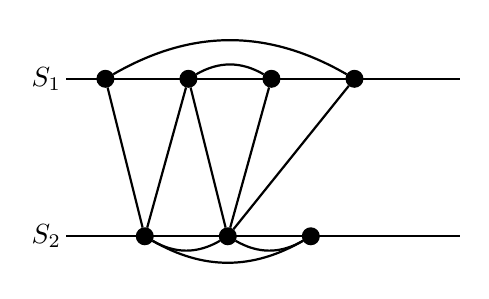
\begin{tikzpicture}

\draw (0, 0) node[left] {$S_2$} -- (5, 0);
\draw (0, 2) node[left] {$S_1$} -- (5, 2);

\tikzstyle{every node}+=[circle,draw,fill]

\node[circle,draw] (o1) at (1, 0) {};
\node[right of=o1] (o2) {};
\node[right of=o2] (o3) {};

\node (u1) at (0.5, 2) {};
\node[right of=u1] (u2) {};
\node[right of=u2] (u3) {};
\node[right of=u3] (u4) {};

\drawedges[bend right]{o1/o2,o1/o3,o2/o3}
\drawedges{o1/u1,o1/u2,o2/u2,o2/u3,o2/u4}
\drawedges[bend left]{u1/u4,u2/u3}

\end{tikzpicture}
%\newProb{\probMul}{Vertex sets~$V_1$, \dots, $V_k$ and
%edge sets $E_0 \subseteq \binom{V_1}{2}$, $E_1 \subseteq V_1\times V_2$,
%\dots, $E_{k-1} \subseteq V_{k-1} \times V_k$, $E_k \subseteq \binom{V_k}{2}$.}{Is there
%a planar drawing of $(V_1 \cup \dotsb \cup V_k, E_0 \cup \dotsb \cup E_k)$ such that
%a vertex in~$V_i$ lies on~$S_i$ for all~$i \in \range{k}$, edges do not cross a spine,
%the edges in~$E_0$ lie completely above~$S_1$ and the edges in~$E_k$ lie completely below~$S_k$?}
Without caps: Solvable in linear time [Jünger et al., 1999].
\end{frame}

\begin{frame}{Level planarity}
Level planarity is an ordering problem:
\begin{figure}[\placement]
\centering

%\resizebox{\textwidth}{!}{
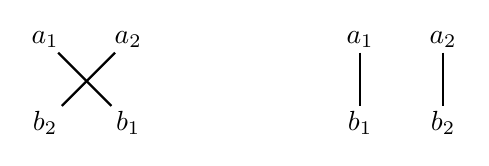
\begin{tikzpicture}

%\tikzstyle{every node}+=[circle,draw]

\node (A1) {$a_1$};
\node[right of=A1] (A2) {$a_2$};
\node[below of=A1] (B2) {$b_2$};
\node[right of=B2] (B1) {$b_1$};
\draw (A1) edge (B1);
\draw (A2) edge (B2);

\begin{scope}[xshift=4cm]
\node (A1) {$a_1$};
\node[right of=A1] (A2) {$a_2$};
\node[below of=A1] (B1) {$b_1$};
\node[right of=B1] (B2) {$b_2$};
\draw (A1) edge (B1);
\draw (A2) edge (B2);
\end{scope}

\end{tikzpicture}
%}
\end{figure}
Forbidden: $a_1 <_i a_2 \land b_2 < b_1$ for $(a_1, b_1), (a_2, b_2) \in E_i$ 
\end{frame}

%\begin{frame}{Observations}
%
%Embeddability only depends on the order of the vertices on the spines:
%\begin{itemize}
%\item Caps come from page embedding
%\item Two edges between TODO
%\end{itemize}
%\end{frame}

\begin{frame}{Mapping to 2-page \probPTree}

\begin{theorem}
A \probMul instance is equivalent to a special 2-page \probPTree instance.
\end{theorem}

\begin{figure}[\placement]
\centering

\resizebox{0.90\textwidth}{!}{
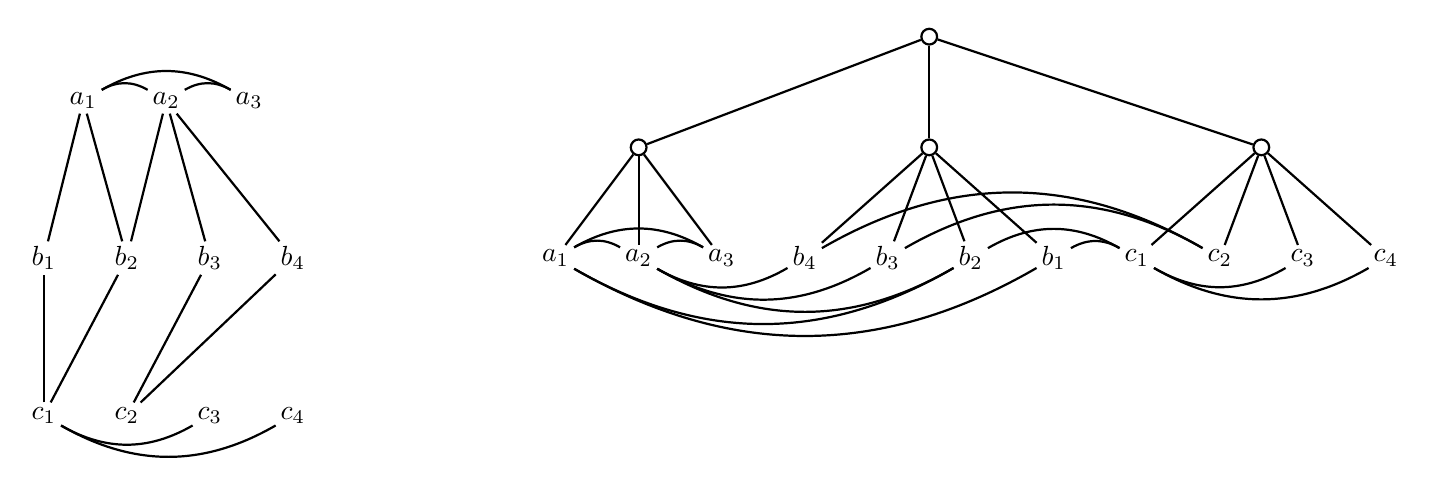
\begin{tikzpicture}

%\draw (0, 0) node[left] {} -- (5, 0);
%\draw (0, -2) node[left] {} -- (5, -2);

%\tikzstyle{every node}+=[circle,draw,fill]

\node (a1) at (1, 0) {$a_1$};
\node[right of=a1] (a2) {$a_2$};
\node[right of=a2] (a3) {$a_3$};

\node (b1) at (0.5, -2) {$b_1$};
\node[right of=b1] (b2) {$b_2$};
\node[right of=b2] (b3) {$b_3$};
\node[right of=b3] (b4) {$b_4$};

\node (c1) at (0.5, -4) {$c_1$};
\node[right of=c1] (c2) {$c_2$};
\node[right of=c2] (c3) {$c_3$};
\node[right of=c3] (c4) {$c_4$};


\drawedges[bend left]{a1/a2,a1/a3,a2/a3}
\drawedges{a1/b1,a1/b2,a2/b2,a2/b3,a2/b4}
\drawedges{c1/b1,c1/b2,c2/b3,c2/b4}
\drawedges[bend right]{c1/c4,c1/c3}

\node[draw=none,fill=none] at (5.5,-2) {{\Huge $\rightsquigarrow$}};

\begin{scope}[xshift=7cm,yshift=-2cm]

%\draw (-1, 0) -- (9, 0);

\node (a1) at (0, 0) {$a_1$};
\node[right of=a1] (a2) {$a_2$};
\node[right of=a2] (a3) {$a_3$};

\node[right of=a3] (b4) {$b_4$};
\node[right of=b4] (b3) {$b_3$};
\node[right of=b3] (b2) {$b_2$};
\node[right of=b2] (b1) {$b_1$};

\node[right of=b1] (c1) {$c_1$};
\node[right of=c1] (c2) {$c_2$};
\node[right of=c2] (c3) {$c_3$};
\node[right of=c3] (c4) {$c_4$};

\drawedges[bend left]{a1/a2,a1/a3,a2/a3}
\drawedges[bend right]{a1/b1,a1/b2,a2/b2,a2/b3,a2/b4}
\drawedges[bend right]{c1/b1,c1/b2,c2/b3,c2/b4}
\drawedges[bend right]{c1/c4,c1/c3}

\end{scope}

\visible<2->{
\node[circle, draw] (r1) at ($ (a2) + (0, 4em) $) {};
\node[circle, draw] (r2) at ($ 0.5*($ (b2) + (b3) $) + (0, 4em)$) {};
\node[circle, draw] (r3) at ($ 0.5*($ (c2) + (c3) $) + (0, 4em)$) {};
\node[circle, draw] (r) at ($ (r2) + (0, 4em) $) {};
\drawedges[ultra thick]{r1/a1,r1/a2,r1/a3,r2/b1,r2/b2,r2/b3,r2/b4,r3/c1,r3/c2,r3/c3,r3/c4,r/r1,r/r2,r/r3}
}

\end{tikzpicture}
}
\end{figure}

\end{frame}

\miniframesoff

%\begin{frame}{The end}
%
%\begin{center}
%\large{Thank you for your attention.}
%\end{center}
%
%\vfill
%\small{I would also like to thank my advisors Dipl.-Inform. Thomas Bläsius and
%Dr. Ignaz Rutter for all their continued support, guidance, advice as well
%as for the insightful discussions I had with them.}
%
%\end{frame} 

\begin{frame}{Conclusion and outlook}
\begin{overprint}
\onslide<1>\solutionTri{1}{0.6\textwidth}
\onslide<2>\solutionTri{2}{0.6\textwidth}
\onslide<3>\solutionTri{3}{0.6\textwidth}
\onslide<4>\solutionTri{4}{0.6\textwidth}
\onslide<5>\solutionTri{5}{0.6\textwidth}
\onslide<6>\solutionTri{6}{0.6\textwidth}
\vspace{-1.8em}
\begin{itemize}
  \item Complexity for constant number of pages?
  \item Complexity when constrained by a \PT-tree?
\end{itemize}

\end{overprint}
\end{frame}

\begin{frame}{Addendum: Multiple spines}
\begin{figure}[\placement]
\centering

\resizebox{0.90\textwidth}{!}{
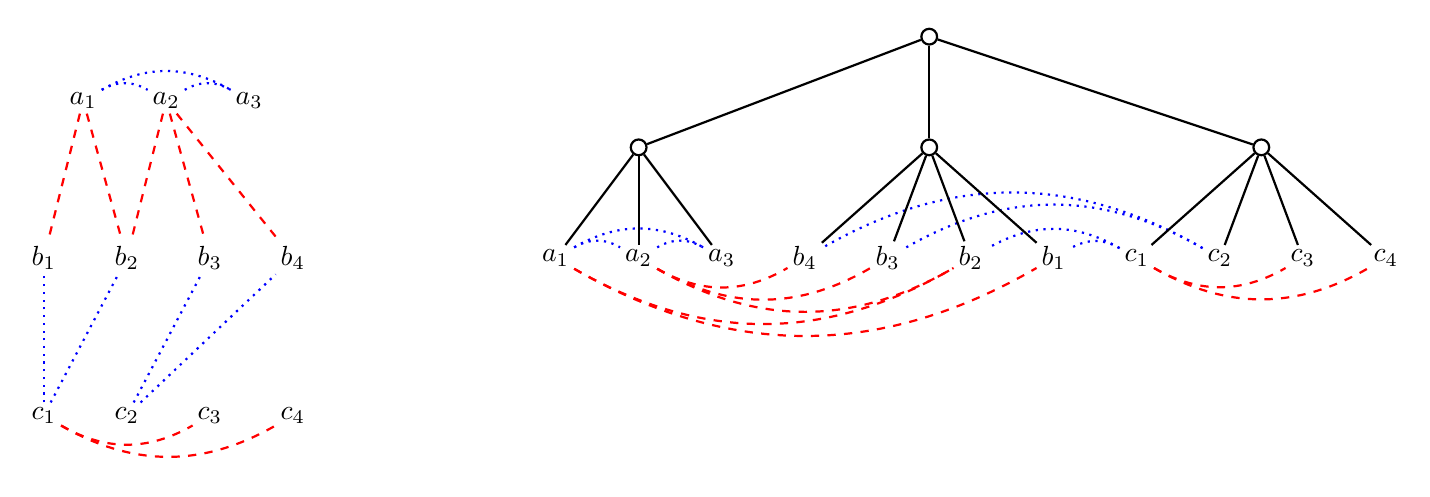
\begin{tikzpicture}

%\draw (0, 0) node[left] {} -- (5, 0);
%\draw (0, -2) node[left] {} -- (5, -2);

%\tikzstyle{every node}+=[circle,draw,fill]

\node (a1) at (1, 0) {$a_1$};
\node[right of=a1] (a2) {$a_2$};
\node[right of=a2] (a3) {$a_3$};

\node (b1) at (0.5, -2) {$b_1$};
\node[right of=b1] (b2) {$b_2$};
\node[right of=b2] (b3) {$b_3$};
\node[right of=b3] (b4) {$b_4$};

\node (c1) at (0.5, -4) {$c_1$};
\node[right of=c1] (c2) {$c_2$};
\node[right of=c2] (c3) {$c_3$};
\node[right of=c3] (c4) {$c_4$};


\drawedges[bend left,edge2]{a1/a2,a1/a3,a2/a3}
\drawedges[edge1]{a1/b1,a1/b2,a2/b2,a2/b3,a2/b4}
\drawedges[edge2]{c1/b1,c1/b2,c2/b3,c2/b4}
\drawedges[bend right,edge1]{c1/c4,c1/c3}

\node[draw=none,fill=none] at (5.5,-2) {{\Huge $\rightsquigarrow$}};

\begin{scope}[xshift=7cm,yshift=-2cm]

%\draw (-1, 0) -- (9, 0);

\node (a1) at (0, 0) {$a_1$};
\node[right of=a1] (a2) {$a_2$};
\node[right of=a2] (a3) {$a_3$};

\node[right of=a3] (b4) {$b_4$};
\node[right of=b4] (b3) {$b_3$};
\node[right of=b3] (b2) {$b_2$};
\node[right of=b2] (b1) {$b_1$};

\node[right of=b1] (c1) {$c_1$};
\node[right of=c1] (c2) {$c_2$};
\node[right of=c2] (c3) {$c_3$};
\node[right of=c3] (c4) {$c_4$};

\drawedges[bend left,edge2]{a1/a2,a1/a3,a2/a3}
\drawedges[bend right,edge1]{a1/b1,a1/b2,a2/b2,a2/b3,a2/b4}
\drawedges[bend right,edge2]{c1/b1,c1/b2,c2/b3,c2/b4}
\drawedges[bend right,edge1]{c1/c4,c1/c3}

\end{scope}

\node[circle, draw] (r1) at ($ (a2) + (0, 4em) $) {};
\node[circle, draw] (r2) at ($ 0.5*($ (b2) + (b3) $) + (0, 4em)$) {};
\node[circle, draw] (r3) at ($ 0.5*($ (c2) + (c3) $) + (0, 4em)$) {};
\node[circle, draw] (r) at ($ (r2) + (0, 4em) $) {};
\drawedges[ultra thick]{r1/a1,r1/a2,r1/a3,r2/b1,r2/b2,r2/b3,r2/b4,r3/c1,r3/c2,r3/c3,r3/c4,r/r1,r/r2,r/r3}

\end{tikzpicture}
}
\end{figure}
\end{frame}

\end{document}
